\subsection{$w_0~w_a$ constraints}

\myparagraph{Method}

In order to assess the impact of the cadence on the cosmological analysis possible with supernovae, we compute the Dark Energy Task force figure of merit in the dark energy parameters $w_0-w_a,$ for a few scenarios.
In the first instance, the supernova sample is simulated following roughly the same prescription as that outlined in the recent Science Requirements Document \cite{descsrd}, with small changes to the host redshift selection. For the SRD we adjusted the survey size simulated to ensure roughly 112 000 SNe after host selection cuts from a 4MOST-like ground based telescope. This is the largest determinant of the final size, and so in order to test for differences in the survey strategy we initially doubled the survey size simulated, and then tested a few cadences without requiring any spectrosopic host redshift. This was to ensure that the host-$z$ follow up was not the most important characteristic.
In addition, we imposed a more restrictive cut on the fitted colour in the SAL2T fit from $\sigma(c) < 0.08$ to $\sigma(c) < 0.05.$ Insodoing we are forcing that the supernovae that survive are of higher quality than in the DESC SRD.
Finally, we include only statistical errors: for speed of computation we have neglected the astrophysical systematics; this will be relaxed in future versions

\myparagraph{Results}

\begin{figure}
  \begin{center}
  \subfigure[w0-wa ellipses]{\label{fig:w0wa}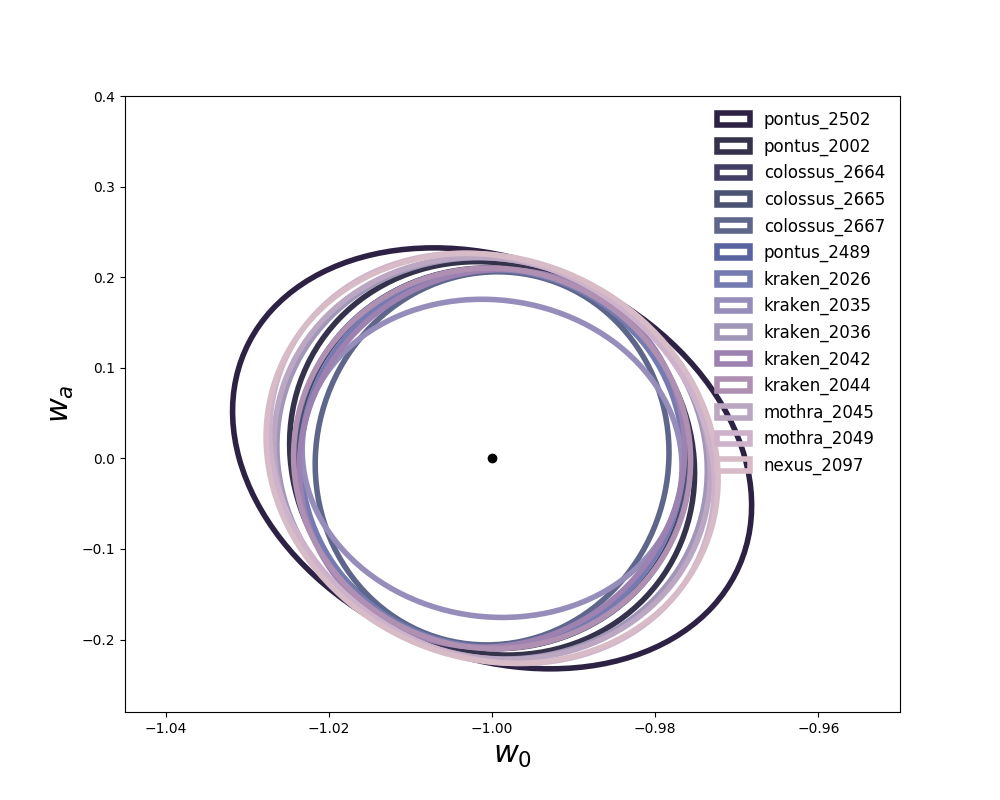
\includegraphics[width=0.7\textwidth]{w0wa/FM_plot_cadence_updated.png}}
    \subfigure[FoM vs observing strategy]{\label{fig:snfom}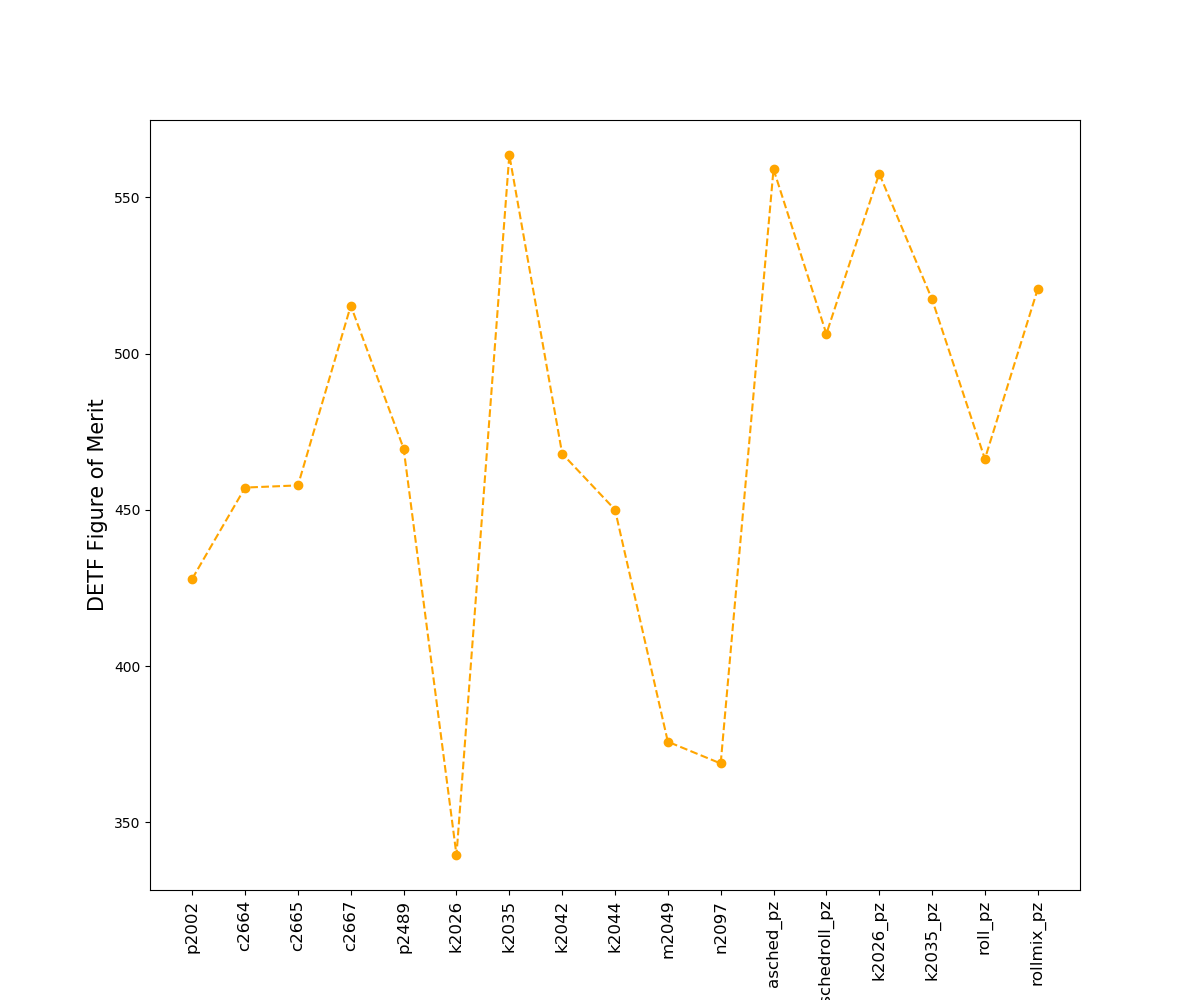
\includegraphics[width=0.7\textwidth]{w0wa/FoM_cadence_updated.png}}
    \caption{Cosmology constraints across cadence types: the ellipses in the $w_0-w_a$ plane (a) and the dark energy figure of merit is shown (b) are shown. \textbf{[RH: plot to be changed once NSERC comes back online 10/18]}}
    \end{center}
\end{figure}

In the figgure above, we see that the largest difference in the Figure of Merit \ref{fig:w0wa} we find is a factor of two between the highest FoM (kraken\_2035) and the lowest FoM (pontus\_2502). The lowest-performing strategy has two alternating bands in declination, switching in alternate years, which is expect to perform poorly. 

In order to test more strongly the impact of the wide field cadence on the overall cosmology, we ran simulations including \textit{only the WFD survey} in addition to a low-$z$ (e.g. Foundation-like) data set. We compared the cosmology results from the WFD+Foundation surveys for the {\tt kraken_2026, kraken_2035} and {\tt altsched, altsched_rolling} cadences. Finally we show the results with and without spectroscopic host redshift selection for the baseline {\tt kraken_2026} survey. \textbf{[RH: these cosmosis runs will proceed on NSERC on 10/18 after cori comes back up]}

\myparagraph{Conclusion}

